\documentclass[11pt, a4paper]{article}

% --- Packages ---
\usepackage[utf8]{inputenc}
\usepackage[T1]{fontenc}
\usepackage{mathptmx} % Professional Times New Roman typography
\usepackage{graphicx}
\usepackage[margin=0.8in]{geometry}
\usepackage{xcolor}
\usepackage{titlesec}
\usepackage{enumitem}
\usepackage{float}
\usepackage{booktabs}
\usepackage{multirow}
\usepackage{array}
\usepackage{hyperref}
\graphicspath{{figures/}}

\hypersetup{
    colorlinks=true,
    linkcolor=amritaMaroon,
    citecolor=amritaMaroon,
    urlcolor=blue
}

% --- Amrita Colors ---
\definecolor{amritaMaroon}{HTML}{A4123F}

% --- Title & Section Formatting ---
\titlespacing*{\section}{0pt}{12pt}{4pt}
\titlespacing*{\subsection}{0pt}{8pt}{3pt}
\titleformat{\section}{\large\bfseries\color{amritaMaroon}}{\thesection}{0.8em}{}
\titleformat{\subsection}{\normalsize\bfseries\color{amritaMaroon}}{\thesubsection}{0.6em}{}

\pagestyle{plain}

\begin{document}

% ==========================================
% HEADER & TITLE BLOCK
% ==========================================
\noindent
\begin{minipage}{\textwidth}
    \centering
    {\Large \textbf{\textcolor{amritaMaroon}{
    AMRITA VISHWA VIDYAPEETHAM \\
    SCHOOL OF COMPUTING \\
    DEPARTMENT OF COMPUTER SCIENCE AND ENGINEERING \\
    }}}
    \vspace{0.2cm}
    {\large \textbf{EvoSynth: Dynamic Multi-Armed Bandit Meta-Optimizer for Automated Model Selection and Hyperparameter Tuning}} \\[0.1cm]
    \textbf{23CSE498 -- Project Phase II (External Review)} \quad | \quad \textbf{Team Number: 2} \\
    \today
\end{minipage}

\vspace{0.3cm}
\hrule
\vspace{0.3cm}

% --- Team & Guide Details ---
\noindent
\begin{center}
    \renewcommand{\arraystretch}{1.35}
    \setlength{\tabcolsep}{6pt}
    \begin{tabular}{|l|p{4.8cm}|p{4.6cm}|p{3.2cm}|}
        \hline
        \multicolumn{2}{|c|}{\textbf{Team Members}} & \textbf{Project Guide} & \textbf{Project Type} \\
        \hline
        \small CB.SC.U4CSE23445 & \small \raggedright Shivam Kharat &
        \multirow{5}{=}{\raggedright \small \textbf{Dr. Thangavelu S.} \newline \textit{Associate Professor, \newline Dept. of CSE}} &
        \multirow{5}{=}{\raggedright \small \textbf{Type 1} \newline Research-Based Project} \\ \cline{1-2}
        \small CB.SC.U4CSE23565 & \small Siddharth Ladda & & \\ \cline{1-2}
        \small CB.SC.U4CSE23627 & \small Kaushal Loya & & \\ \cline{1-2}
        \small CB.SC.U4CSE23639 & \small Paarthu Reddy & & \\ \cline{1-2}
        \small CB.SC.U4CSE23642 & \small Priyansh Narang & & \\
        \hline
    \end{tabular}
\end{center}
\vspace{0.2cm}

\section{Abstract}
\noindent
Automated Machine Learning (AutoML) seeks to remove manual trial-and-error by automatically searching for optimal machine learning pipelines. However, contemporary frameworks (e.g., Optuna \cite{akiba2019optuna}, FLAML \cite{wang2021flaml}, and H2O AutoML \cite{ledell2020h2o}) rely on a single, fixed search algorithm throughout the optimization lifetime. As established by the No Free Lunch theorem \cite{wolpert1997no}, no single optimization heuristic consistently dominates across complex, rugged, and non-convex hyperparameter landscapes, causing static systems to stagnate. Furthermore, post-hoc ensembling methods achieve high accuracy only by stacking numerous large models, resulting in prohibitively high inference latencies and severe cloud memory footprints. 

To overcome these fundamental challenges, this research presents \textbf{EvoSynth}, a dynamic multi-armed bandit meta-optimizer for automated model selection and hyperparameter optimization. EvoSynth maps mixed continuous, discrete, and categorical hyperparameters into a unified mathematical latent space $[0,1]^d$. It concurrently coordinates four diverse evolutionary and metaheuristic optimizers: Genetic Algorithms (GA) \cite{holland1975adaptation}, Particle Swarm Optimization (PSO) \cite{kennedy1995particle}, Differential Evolution (DE) \cite{storn1997differential}, and Covariance Matrix Adaptation Evolution Strategy (CMA-ES) \cite{hansen2001completely}. A UCB1 \cite{auer2002finite} multi-armed bandit meta-engine monitors a 5-metric composite reward (fitness, speed, efficiency, population diversity, and improvement trend) to dynamically allocate evaluations and execute live tier promotion, demotion (SWAPs), and rollback safeguards across a two-tier island topology \cite{alba2002parallelism}. After the search, the five best distinct configurations are re-scored with 5-fold cross-validation and the selected one is refitted once and scored once on held-out test rows. Under an identical protocol on UCI Covertype \cite{blackard1999comparative} (581,012 samples, 7 classes) and Adult \cite{kohavi1996scaling} (48,842 samples, binary), EvoSynth reached \textbf{93.89\% test accuracy} and \textbf{92.96 ROC AUC} with 500 evaluations, level with Random Search \cite{bergstra2012random} and Optuna TPE \cite{bergstra2011algorithms} (within 0.03 points), 1.4 points above FLAML on Covertype and 0.17 below it on Adult, while selecting a different model family for each dataset (ExtraTrees \cite{geurts2006extremely} with interaction features, and XGBoost \cite{chen2016xgboost}). In an optimizer ablation it matched the best single optimizer without knowing in advance which one that would be, and parallel evaluation gave a measured \textbf{6.1$\times$} speed-up. EvoSynth delivers a single model, whose serving cost is that of the selected family (0.26\,ms per row for the Adult XGBoost, 12.5\,ms for the Covertype ExtraTrees).

% --- 2. PROBLEM DEFINITION, MOTIVATION & LITERATURE SURVEY ---
\section{Problem Definition, Research Motivation \& Literature Review}

\subsection{Problem Statement \& Research Motivation}
\begin{itemize}[noitemsep, topsep=2pt]
    \item \textbf{Problem Statement:} Traditional AutoML frameworks \cite{feurer2019hyperparameter, bischl2023hyperparameter} employ static search strategies (e.g., standard Bayesian Optimization \cite{hutter2011sequential}, single-sampler TPE \cite{bergstra2011algorithms}, or localized greedy descent) that cannot adapt when encountering local optima, deceptive plateaus, or non-convex topological shifts. Consequently, significant computational budgets are squandered evaluating suboptimal regions using an underperforming algorithm.
    \item \textbf{Research Motivation:} In production and edge environments, machine learning solutions must balance accuracy against deployment practicality. Existing solutions that produce large ensemble stacks introduce unsustainable inference latencies and memory footprints. There is a critical need for an adaptive meta-optimizer that dynamically detects search stagnation, swaps optimization strategies during runtime, and delivers a single, highly tuned standalone model.
    \item \textbf{Research Objectives:}
    \begin{enumerate}[noitemsep, topsep=2pt]
        \item \textbf{Dynamic Multi-Armed Bandit Allocation:} Formulate a UCB1 meta-engine capable of dynamically scoring and allocating computational budget across competing optimization heuristics.
        \item \textbf{Stagnation-Resilient Two-Tier Architecture:} Implement an adaptive island model with automated promotion, live demotion (SWAP), rollback safeguards, and diversity injection to escape deceptive search landscapes.
        \item \textbf{Fair, Reproducible Evaluation:} Compare against untuned models, Random Search, Optuna and FLAML on real datasets with fixed held-out test rows and an identical selection and refit, delivering a single deployable model with measured inference cost.
    \end{enumerate}
\end{itemize}

\subsection{Literature Review \& Research Gap}
\noindent
Recent advances in automated machine learning and metaheuristic optimization highlight both the potential of automated pipelines and the systemic drawbacks of static search frameworks.

\begin{table}[H]
    \centering
    \footnotesize
    \renewcommand{\arraystretch}{1.25}
    \begin{tabular}{|p{3.2cm}|p{4.2cm}|p{4.0cm}|p{3.8cm}|}
        \hline
        \textbf{Author / Year / Citation} & \textbf{Core Methodology Used} & \textbf{Key Findings / Strengths} & \textbf{Identified Limitations} \\
        \hline
        Franceschi et al. (2025) \cite{franceschi2025hyperparameter} & Monograph on HPO: random, bandit, model-, population- and gradient-based methods. & Unified treatment of HPO families and open problems. & Survey only; no new method or experiments. \\
        \hline
        Alcoba\c{c}a \& Carvalho (2026) \cite{alcobaca2026literature} & Systematic review of AutoML literature reviews (meta-learning, HPO, transfer). & Organizes the field and its research directions. & Survey only; no dynamic switching between optimizers within a run. \\
        \hline
        Guo et al. (2024) \cite{guo2024deep} (RL-DAS) & Deep RL agent switches among DE variants during a run, with context restoration. & Dynamic switching improves overall optimization performance and generalizes across problem classes. & Needs offline agent training; tested on benchmark functions, not ML pipelines. \\
        \hline
        \v{C}repin\v{s}ek et al. (2025) \cite{crepinsek2025overcoming} (MsMA) & Meta-level wrapper that reallocates a metaheuristic's budget when progress stalls. & Improved every tested algorithm on CEC'24 and a real load-flow problem. & Wraps one algorithm at a time; theoretical benchmark functions rather than AutoML. \\
        \hline
        Ma et al. (2025) \cite{ma2025toward} & Survey and benchmark of meta-black-box optimization (learned algorithm selection/configuration). & Taxonomy of selection, configuration and generation; identifies designs that generalize. & Learned controllers must be trained offline on a distribution of problems. \\
        \hline
        Benjamins et al. (2025) \cite{benjamins2025carps} (carps) & Framework to compare $N$ HPO optimizers on $M$ benchmark tasks. & 3336 tasks and 26 optimizer variants; representative task subsets. & Benchmarks optimizers one at a time; no online portfolio among them. \\
        \hline
        Rezaei Balef et al. (2025) \cite{balef2025cash} (MaxUCB) & Max $k$-armed bandit over model classes, each with its own HPO run, for CASH. & Outperforms combined search and prior bandit methods on four AutoML benchmarks; theoretical analysis. & Arms are model classes with one fixed tuner each; assumes stationary rewards. \\
        \hline
        Schneider et al. (2025) \cite{schneider2025overtuning} & Large-scale reanalysis of HPO benchmark data for overtuning. & Overtuning is common; in about 10\% of cases the chosen configuration is worse than the default. & Motivates, but does not provide, a remedy such as re-scoring the top candidates. \\
        \hline
        Nagler et al. (2024) \cite{nagler2024reshuffling} & Theory and experiments on reshuffling resampling splits during HPO. & Reshuffling makes cheap holdout competitive with cross-validation. & The selection protocol still matters; fixed splits can overfit the validation data. \\
        \hline
        Erickson et al. (2025) \cite{erickson2025tabarena} (TabArena) & Living benchmark of 16 tabular models on 51 datasets. & Tuning plus post-hoc ensembling gives the best tabular accuracy. & Ensembles add inference cost; single-model deployment is not the focus. \\
        \hline
    \end{tabular}
    \caption{Summary of Key Literature Surveyed and Identified Limitations}
\end{table}

\noindent
\textbf{Summary of Research Gap:} Recent work allocates HPO budget among model classes with a bandit (MaxUCB \cite{balef2025cash}), switches among evolutionary algorithms with an offline-trained agent (RL-DAS \cite{guo2024deep}), or reallocates the budget of a single stalled metaheuristic (MsMA \cite{crepinsek2025overcoming}); AutoML systems either commit to one search strategy (FLAML) or ensemble many models (H2O, TabArena \cite{erickson2025tabarena}). No applied AutoML system runs several distinct evolutionary optimizers concurrently on one joint CASH space \cite{thornton2013autoweka}, reallocates budget among them online without offline training, promotes, swaps and rolls them back, and delivers a single confirmed model whose selection guards against overtuning \cite{schneider2025overtuning, nagler2024reshuffling}.

% --- 3. PROPOSED METHODOLOGY & SOLUTION DESIGN ---
\section{Proposed Methodology \& Solution Design}

\subsection{End-to-End Methodological Workflow}
\noindent
EvoSynth adopts a fully decoupled architecture separating search heuristics from machine learning model evaluation through a unified mathematical latent space. The workflow progresses from parameter encoding to tournament evaluation, dynamic selection, exploitation, confirmation of the best candidates, and a single refit scored on held-out test rows.

\begin{figure}[H]
    \centering
    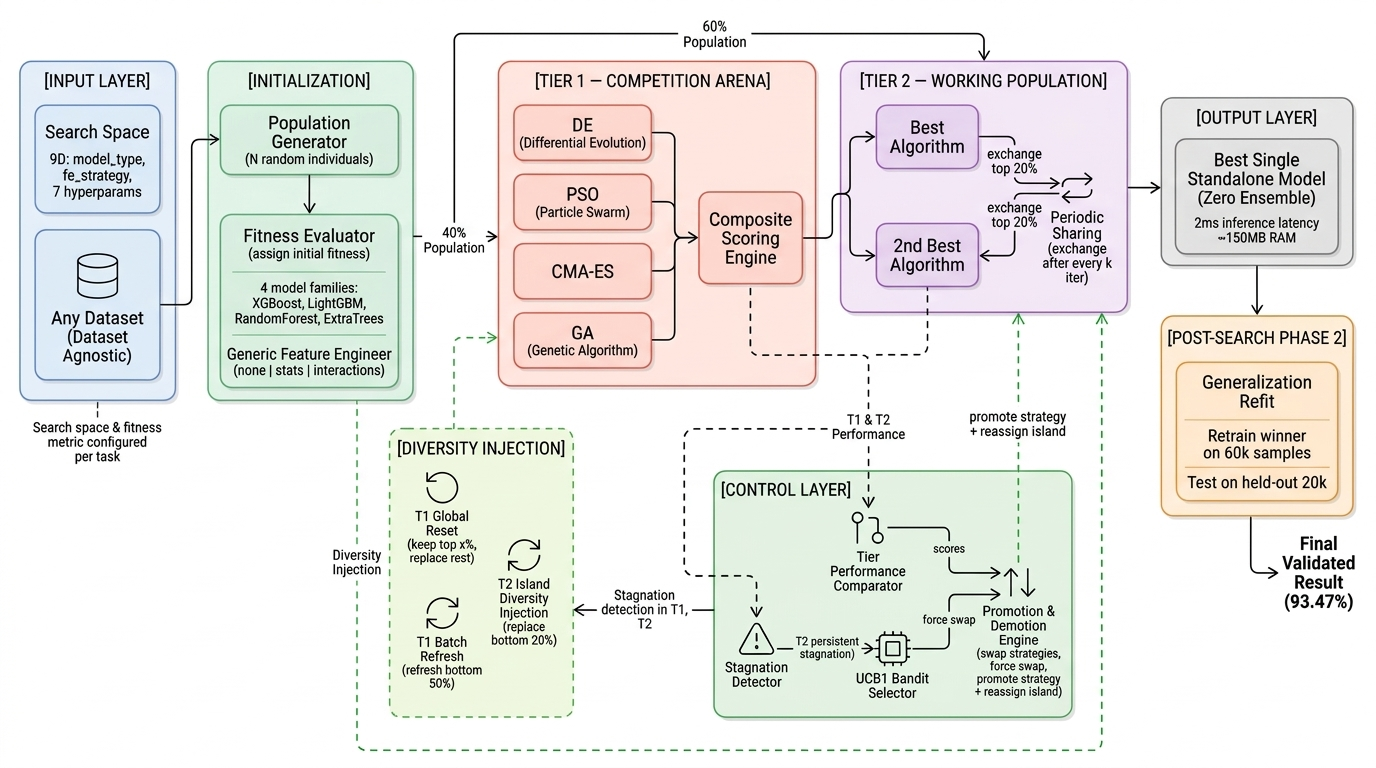
\includegraphics[width=0.92\textwidth, height=6.2cm, keepaspectratio]{arch.png}
    \caption{EvoSynth System Architecture: input layer, stratified 40/60 population split, Tier 1 tournament (four islands of $N/10$), composite scoring and UCB1 control layer, Tier 2 working population with elite sharing and diversity injection, and single-model output after confirmation and refit.}
\end{figure}

\subsection{Mathematical Formulation \& Algorithmic Design}
\begin{itemize}[noitemsep, topsep=2pt]
    \item \textbf{Latent Space Normalization:} Any heterogeneous search space $\Theta$ containing continuous, discrete, and categorical parameters is bijectively transformed into a continuous unit hypercube $\mathcal{Z} = [0, 1]^d$. Categorical choices (e.g., model architecture and feature engineering strategies) with $K$ discrete options are discretized via uniform intervals: $k = \min(\lfloor z_j \cdot K \rfloor, K-1)$.
    \item \textbf{Composite Scoring Engine ($CS_i$):} Rather than evaluating candidate algorithms purely on single best accuracy, EvoSynth evaluates five normalized operational dimensions:
    \begin{equation}
        CS_i = 0.30 \cdot F_i + 0.25 \cdot S_i + 0.15 \cdot E_i + 0.15 \cdot D_i + 0.15 \cdot T_i
    \end{equation}
    where $F_i$ is the family's best cross-validated score, $S_i$ (speed) is the improvement of that best since the family's previous scoring call, $E_i$ (efficiency) is that improvement per second of evaluation time, $D_i$ is the mean pairwise distance between the island's latent vectors divided by $\sqrt{d}$, and $T_i$ (trend) is the slope of the best score over the last three scoring calls. Each term is min-max normalised across the competing families before weighting.
    \item \textbf{Budget-Constrained UCB1 Bandit Allocation:} Computational evaluations are treated as budget pulls routed according to:
    \begin{equation}
        UCB_i = CS_i + c \sqrt{\frac{\ln(E_{\text{total}})}{E_i}}
    \end{equation}
    where $E_{\text{total}}$ is total evaluations consumed across all algorithms, $E_i$ is evaluations allocated to algorithm $i$, and $c=0.1$ balances exploitation with exploration.
    \item \textbf{Two-Tier Island Strategy \& Live SWAP Protocol:} 
    \begin{itemize}[noitemsep]
        \item \textit{Tier 1 (Competition Arena):} A stratified draw gives 40\% of the initial population of size $N$ to four equal islands of $N/10$, one per optimizer (GA, PSO, DE, CMA-ES), so every island holds a mix of strong and weak members. The other 60\% is held in reserve in two groups.
        \item \textit{Tier 2 (Working Exploitation):} The two families with the highest UCB scores after the tournament are promoted; each takes one reserve group. At every checkpoint the two Tier 2 islands trade elites pairwise (each one's worst 20\% replaced by the other's best 20\%). Stagnant islands receive random members through the optimizer's \texttt{inject} method: 50\% at once in Tier 1, 20\% after three stagnant checkpoints in Tier 2.
        \item \textit{Dynamic SWAP \& Rollback:} If the best Tier 1 family's UCB score exceeds the weaker Tier 2 family's by more than an additive margin of 0.10, the two are swapped. If the promoted family does not improve the global best within a 5-iteration grace period, the swap is rolled back from a saved snapshot. Every promotion, swap, rollback, injection and elite exchange is recorded in the run's decision log.
    \end{itemize}
    \item \textbf{Search Space \& Evaluator:} The tabular search space has 8 dimensions: model family (\textit{XGBoost} \cite{chen2016xgboost}, \textit{LightGBM} \cite{ke2017lightgbm}, \textit{RandomForest} \cite{breiman2001random}, \textit{ExtraTrees} \cite{geurts2006extremely}), feature-engineering strategy (\textit{none, stats, interactions}), and 6 numeric hyperparameters (learning rate, number of estimators, maximum depth, subsample ratio, column-sample ratio, and L1 regularisation). Each candidate is scored by stratified 2-fold cross-validation on the dataset's search rows, in the dataset's own metric (accuracy or ROC AUC); gradient-boosted models stop early on a 15\% slice of the training fold.
    \item \textbf{Confirm Before Select:} Search scores from 2-fold CV are noisy and biased upwards by selection \cite{schneider2025overtuning, nagler2024reshuffling}. After the search, the 5 best distinct configurations are re-scored with 5-fold CV and the best confirmed configuration is selected.
\end{itemize}

% --- 4. COMPLETE IMPLEMENTATION DETAILS (100%) ---
\section{Implementation Details}

\subsection{Implementation Environment \& Execution Setup}
\begin{itemize}[noitemsep, topsep=2pt]
    \item \textbf{Hardware \& Compute Specifications:} Standard multi-core personal computer (AMD/Intel 8-core CPU, 16\,GB RAM, standard SSD storage). No specialized GPU acceleration was required for tabular optimization, proving computational accessibility.
    \item \textbf{Software \& Libraries:} Python 3.14, Scikit-Learn 1.6+ \cite{pedregosa2011scikit}, XGBoost 2.1+, LightGBM 4.5+, PyTorch 2.5+ \cite{paszke2019pytorch}, Optuna and FLAML (baselines), FastAPI, React 19, and Vite.
    \item \textbf{Source Code Repository:} Public GitHub repository maintained at \url{https://github.com/paarthureddy/EvoSynth} (active development branch: \texttt{PostReview2}), complete with continuous documentation at \url{https://evosynth-2027.github.io/evosynth-docs/} and benchmark dataset archiving on Zenodo (EvoSynth-Bench v2.0.0, DOI: 10.5281/zenodo.23645119).
\end{itemize}

\subsection{Module-Wise Implementation \& Integration Summary}
\begin{table}[H]
    \centering
    \footnotesize
    \renewcommand{\arraystretch}{1.25}
    \begin{tabular}{|p{3.8cm}|p{7.5cm}|c|}
        \hline
        \textbf{Module / Stage} & \textbf{Implemented Technical Details \& Integration Scope} & \textbf{Status} \\
        \hline
        Latent Space Translator & Mathematical continuous-to-mixed parameter encoding/decoding engine with discrete binning. & 100\% (Integrated) \\
        \hline
        Worker Optimizers & Ask/Tell wrappers implementing Genetic Algorithm, PSO, Differential Evolution, and CMA-ES. & 100\% (Integrated) \\
        \hline
        UCB1 Meta-Engine & Dynamic multi-armed bandit controller with composite reward calculation, promotion, and SWAP. & 100\% (Integrated) \\
        \hline
        Tier Manager \& Safeguards & Stratified 40/60 population allocation, pairwise top-20\% elite sharing, rollback with cooldowns, and diversity injection. & 100\% (Integrated) \\
        \hline
        Generic Feature Engineer & Dataset-agnostic transformer generating statistical aggregations and pairwise interactions. & 100\% (Integrated) \\
        \hline
        Datasets \& Evaluators & Eight real datasets (Covertype, HIGGS, Adult, Airlines, Poker Hand, MiniBooNE, Jannis, Fashion-MNIST \cite{xiao2017fashion}) with fixed test / search / train rows; cross-validated evaluation of the four tree families and a CNN evaluator for NAS \cite{zoph2016neural}. & 100\% (Functional) \\
        \hline
        Selection, Refit \& Inference & Confirm-before-select, one shared refit for EvoSynth, Random Search and Optuna, held-out test scoring, and measurement of single-row latency, throughput and model size. & 100\% (Integrated) \\
        \hline
        Experiment Harness & Baselines (untuned defaults, Random Search, Optuna TPE, FLAML), optimizer ablation, parallel speed-up benchmark, and a resumable experiment runner with summary tables. & 100\% (Integrated) \\
        \hline
        Telemetry \& Live UI & Non-blocking FastAPI SSE event streamer publishing telemetry to a responsive React Vite dashboard. & 100\% (Integrated) \\
        \hline
    \end{tabular}
    \caption{Module-Wise Implementation Completion Status}
\end{table}

\subsection{Detailed Module Descriptions}
\begin{itemize}[noitemsep, topsep=2pt]
    \item \textbf{Automated Generic Feature Engineering:} To remain strictly dataset-agnostic without manual human domain engineering, the \texttt{GenericFeatureEngineer} operates directly on numerical matrix characteristics. The \texttt{stats} strategy appends row-wise mean, standard deviation, maximum, minimum, and skewness; the \texttt{interactions} strategy dynamically generates top interaction cross-products based on initial feature variance.
    \item \textbf{Population Trajectory Logging \& Reproducibility:} The engine writes structured CSV records (\texttt{warmup\_population.csv}, \texttt{tier1\_population.csv}, and \texttt{tier2\_population.csv}) capturing evaluation ID, algorithm origin, fitness, and parameter vectors, together with the scoring history and decision log. Every random number generator is seeded from the run seed, so a run can be repeated exactly.
    \item \textbf{Held-out Generalization Workflow:} Each dataset is split once: test rows are set aside first and never seen during search or selection; search rows (20,000 for Covertype) are used for cross-validation; train rows (60,000 for Covertype) are used for the refit. The selected configuration is refitted once on the train rows and scored once on the 20,000 test rows. Random Search and Optuna use exactly the same selection and refit, so all tuned methods are compared on equal terms. The exact row indices are published in EvoSynth-Bench v2.0.0.
\end{itemize}

% --- 5. PRELIMINARY VERIFICATION, RESULTS & DEMONSTRATION ---
\section{Preliminary Verification, Experimental Results \& Demonstration}

\subsection{Quantitative Evaluation \& Baseline Comparison}
\noindent
Protocol: test rows are split off first (Covertype 20,000; Adult 12,000) and scored once at the end; searches use a fixed 10,000-row subset of the search rows with 2-fold CV; the selected configuration is refitted on the train rows (Covertype 60,000; Adult 36,000). EvoSynth, Random Search and Optuna TPE each have 500 evaluations and the same confirm-and-refit; FLAML gets the wall time EvoSynth used. All results are from one seed (42), so differences of a few hundredths between tuned methods are ties.

\begin{table}[H]
    \centering
    \footnotesize
    \renewcommand{\arraystretch}{1.25}
    \begin{tabular}{|p{3.6cm}|c|c|c|c|p{3.2cm}|}
        \hline
        \multirow{2}{*}{\textbf{Method}} & \multicolumn{2}{c|}{\textbf{Covertype (accuracy \%)}} & \multicolumn{2}{c|}{\textbf{Adult (ROC AUC \%)}} & \multirow{2}{*}{\textbf{Selected model}} \\
        \cline{2-5}
         & \textbf{Test} & \textbf{Search time} & \textbf{Test} & \textbf{Search time} & \\
        \hline
        Untuned XGBoost & 85.58 & -- & 92.70 & -- & \\
        \hline
        Untuned LightGBM & 84.69 & -- & 92.92 & -- & \\
        \hline
        Untuned RandomForest & 89.09 & -- & 90.74 & -- & \\
        \hline
        Untuned ExtraTrees & 89.77 & -- & 89.15 & -- & \\
        \hline
        FLAML (same wall time) & 92.53 & 13.0 min & \textbf{93.13} & 3.0 min & LightGBM / XGBoost \\
        \hline
        Random Search (500) & \textbf{93.89} & 42.4 min & 92.98 & 19.1 min & ExtraTrees / XGBoost \\
        \hline
        Optuna TPE (500) & 93.87 & 49.8 min & 92.95 & 3.3 min & ExtraTrees / XGBoost \\
        \hline
        \textbf{EvoSynth (500)} & \textbf{93.89} & \textbf{12.2 min} & 92.96 & \textbf{3.0 min} & ExtraTrees + interactions / XGBoost \\
        \hline
    \end{tabular}
    \caption{Held-out test scores on Covertype and Adult under an identical protocol}
\end{table}

\noindent
\textbf{Quantitative Findings:}
\begin{itemize}[noitemsep, topsep=2pt]
    \item EvoSynth ties Random Search and Optuna on both datasets (within 0.03 points) and selected the right model family for each. Tuning with model selection is worth 4.1 points over the best untuned model on Covertype but only 0.06 on Adult.
    \item FLAML trails by 1.4 points on Covertype and is best on Adult (+0.17).
    \item EvoSynth's search was 3.5--4$\times$ faster than the sequential baselines on Covertype because it evaluates candidates in parallel; a separate benchmark measured a \textbf{6.1$\times$} speed-up on 12 threads, almost all from parallelism (early stopping alone: 1.17$\times$).
    \item On Covertype the five best configurations decode to the same effective model (trees capped at 150 during the search), so every competent search reaches the same 82.35\% CV plateau; this explains the ties.
\end{itemize}

\subsection{Optimizer Ablation (Covertype, 500 evaluations)}
\noindent
Each optimizer was also run alone with the full budget. Best search CV accuracy at 125 / 500 evaluations: GA 81.53 / 82.21, PSO 82.35 / 82.35, DE 82.13 / 82.34, CMA-ES 81.89 / 82.35, \textbf{EvoSynth 82.08 / 82.35}. EvoSynth matched the best single optimizer at the full budget. The best single optimizer differs between runs (CMA-ES and DE in the earlier ablation, PSO here), so the portfolio's value is reaching the best score without that choice being made in advance.

\subsection{Verification of Core Hypothesis: Live Dynamic SWAP}
\noindent
The Covertype search log shows the meta-decisions working as designed:
\begin{itemize}[noitemsep, topsep=2pt]
    \item \textbf{Promotion:} after 5 Tier 1 iterations, DE (composite 0.961, UCB 1.010) and CMA-ES (UCB 0.466) were promoted. DE had a lower best than CMA-ES but was still improving and had the most diverse island.
    \item \textbf{SWAP:} at the first checkpoint GA, improving quickly from a low score, displaced DE (UCB 0.592 vs 0.369, margin above 0.10); the two Tier 2 islands then traded their top 20\%.
    \item \textbf{Rollback:} GA reached the 82.35\% plateau through CMA-ES's shared elites but did not improve the global best within its 5-iteration grace period, so DE was restored.
    \item \textbf{Outcome:} CMA-ES found the winning ExtraTrees configuration (82.35\% search CV, 84.84\% confirmed, 93.89\% test). On Adult, GA and PSO were promoted, two SWAPs followed, and PSO found the winner.
\end{itemize}

\subsection{Cross-Domain Generality: Vision NAS Demo}
\noindent
The same engine searched CNN architectures on Fashion-MNIST (channels, fully connected units, dropout, activation, optimizer, learning rate), training each candidate for 2 epochs on 10,000 images. With 160 evaluations it reached \textbf{81.8\% validation accuracy}, found by PSO in Tier 2, with no changes to the engine.

% --- 6. TECHNICAL KNOWLEDGE & DESIGN JUSTIFICATION ---
\section{Technical Justification, Design Trade-offs \& Insights}
\begin{itemize}[noitemsep, topsep=2pt]
    \item \textbf{Algorithmic \& Theoretical Justification:} In hyperparameter optimization, the fitness surface is non-stationary and non-differentiable. While local optimizers often become trapped in local basins, evolutionary methods preserve diverse candidate pools. Coupling them through a multi-armed bandit provides formal regret bounds, allocating evaluations where empirical progress is greatest.
    \item \textbf{Computational Complexity \& Trade-offs:} Mapping parameters to a continuous latent space incurs negligible mathematical decoding cost ($\mathcal{O}(d)$ per candidate), while allowing continuous optimizers (PSO, CMA-ES) to seamlessly tune discrete architectures. Performing meta-optimization entirely offline during search ensures zero latency penalty during model inference.
    \item \textbf{Single Model, Measured Cost:} Stacked ensembles such as H2O AutoML run every query through 10 or more models. EvoSynth delivers one model, so serving costs exactly what that model costs, and this is now measured rather than assumed: the Adult XGBoost takes 0.26\,ms per row and 0.4\,MB, while the Covertype ExtraTrees with interaction features takes 12.5\,ms and 470\,MB. The search does not yet trade accuracy for size or latency; a latency-aware objective is future work.
    \item \textbf{Handling Edge Cases \& Boundary Conditions:} (1) \textit{Rollback Guard} reverts a swapped strategy that fails to improve the global best within 5 iterations; (2) \textit{Stagnation Injection} replaces 50\% of a Tier 1 island (immediately) or 20\% of a Tier 2 island (after 3 stagnant checkpoints) with random vectors; (3) \textit{Confirm Before Select} re-scores the top 5 configurations with 5-fold CV, because the maximum of many noisy 2-fold scores is biased upwards; (4) failed CV folds score 0 and are counted, so a crashing configuration can never be selected.
\end{itemize}

% --- 7. CONCLUSION, LIMITATIONS & FUTURE SCOPE ---
\section{Conclusion, Limitations \& Future Scope}
\begin{itemize}[noitemsep, topsep=2pt]
    \item \textbf{Conclusion:} EvoSynth coordinates four evolutionary and swarm optimizers through a two-tier island model and a UCB1 bandit, searching model family, feature engineering and hyperparameters together. Under an identical held-out protocol it matched Random Search and Optuna on Covertype (93.89\%) and Adult (92.96 ROC AUC), chose the right model family for each, matched the best single optimizer in the ablation without knowing it in advance, and was the fastest tuned search on Covertype.
    \item \textbf{Current Limitations:} On these datasets EvoSynth does not beat strong baselines, and FLAML was best on Adult; the results are from a single seed; the Covertype search space has a plateau that every competent method reaches; execution is on a single machine.
    \item \textbf{Future Scope:} (1) multi-seed runs on harder datasets (HIGGS, Poker Hand); (2) comparison with portfolio baselines such as Nevergrad's NGOpt \cite{meunier2022blackbox} on surrogate benchmarks with many tasks; (3) rank-normalised bandit rewards and a latency-aware objective; (4) distributed workers via Ray.
\end{itemize}

% --- 8. DELIVERABLES & TECHNICAL ENRICHMENT SUMMARY ---
\section{Project Deliverables \& Technical Enrichment Summary}
\begin{table}[H]
    \centering
    \footnotesize
    \renewcommand{\arraystretch}{1.2}
    \begin{tabular}{|p{4.2cm}|p{8.0cm}|c|}
        \hline
        \textbf{Deliverable Category} & \textbf{Details / Title / Repository Link} & \textbf{Status} \\
        \hline
        Source Code Repository & Public repository with complete AutoML engine, evaluators, and dashboard: \newline \url{https://github.com/paarthureddy/EvoSynth} & Completed \\
        \hline
        Project Documentation & Comprehensive VitePress documentation website covering architecture and APIs: \newline \url{https://evosynth-2027.github.io/evosynth-docs/} & Completed \\
        \hline
        Benchmark Dataset Archive & EvoSynth-Bench v2.0.0 public dataset release (real datasets and exact splits) hosted on Zenodo: \newline \url{https://doi.org/10.5281/zenodo.23645119} & Completed \\
        \hline
        Individual Certification 1 & Shivam Kharat: \textit{Supervised Machine Learning in Python} (Udemy, 11 Hrs) & Completed \\
        \hline
        Individual Certification 2 & Siddharth Ladda: \textit{Supervised Machine Learning in Python} (Udemy, 11 Hrs) & Completed \\
        \hline
        Individual Certification 3 & Kaushal Loya: \textit{AI and Meta-Heuristics (Combinatorial Optimization) Python} (Udemy, 17.5 Hrs) & Completed \\
        \hline
        Individual Certification 4 & Paarthu Reddy: \textit{AI and Meta-Heuristics (Combinatorial Optimization) Python} (Udemy, 17.5 Hrs) & Completed \\
        \hline
        Individual Certification 5 & Priyansh Narang: \textit{Supervised Machine Learning in Python} (Udemy, 11 Hrs) & Completed \\
        \hline
    \end{tabular}
    \caption{Summary of Completed Project and Technical Enrichment Deliverables}
\end{table}

% --- REFERENCES ---
\vspace{0.2cm}
\begin{thebibliography}{99}
\small

\item[] \textbf{Research Papers}

\bibitem{wolpert1997no} D. H. Wolpert and W. G. Macready, ``No free lunch theorems for optimization,'' \textit{IEEE Trans. Evol. Comput.}, vol. 1, no. 1, pp. 67--82, 1997.

\bibitem{storn1997differential} R. Storn and K. Price, ``Differential evolution -- A simple and efficient heuristic for global optimization over continuous spaces,'' \textit{J. Global Optimization}, vol. 11, no. 4, pp. 341--359, 1997.

\bibitem{hansen2001completely} N. Hansen and A. Ostermeier, ``Completely derandomized self-adaptation in evolution strategies,'' \textit{Evolutionary Computation}, vol. 9, no. 2, pp. 159--195, 2001.

\bibitem{auer2002finite} P. Auer, N. Cesa-Bianchi, and P. Fischer, ``Finite-time analysis of the multiarmed bandit problem,'' \textit{Machine Learning}, vol. 47, no. 2--3, pp. 235--256, 2002.

\bibitem{alba2002parallelism} E. Alba and M. Tomassini, ``Parallelism and evolutionary algorithms,'' \textit{IEEE Trans. Evol. Comput.}, vol. 6, no. 5, pp. 443--462, 2002.

\bibitem{blackard1999comparative} J. A. Blackard and D. J. Dean, ``Comparative accuracies of artificial neural networks and discriminant analysis in predicting forest cover types from cartographic variables,'' \textit{Computers and Electronics in Agriculture}, vol. 24, no. 3, pp. 131--151, 1999.

\bibitem{bergstra2012random} J. Bergstra and Y. Bengio, ``Random search for hyper-parameter optimization,'' \textit{J. Mach. Learn. Res.}, vol. 13, no. 10, pp. 281--305, 2012.

\bibitem{geurts2006extremely} P. Geurts, D. Ernst, and L. Wehenkel, ``Extremely randomized trees,'' \textit{Machine Learning}, vol. 63, no. 1, pp. 3--42, 2006.

\bibitem{bischl2023hyperparameter} B. Bischl \textit{et al.}, ``Hyperparameter optimization: Foundations, algorithms, best practices, and open challenges,'' \textit{WIREs Data Mining and Knowledge Discovery}, vol. 13, no. 2, p. e1484, 2023.

\bibitem{franceschi2025hyperparameter} L. Franceschi \textit{et al.}, ``Hyperparameter optimization in machine learning,'' \textit{Foundations and Trends in Machine Learning}, vol. 18, no. 6, pp. 1054--1201, 2025.

\bibitem{alcobaca2026literature} E. Alcoba\c{c}a and A. C. P. L. F. de Carvalho, ``A literature review on automated machine learning,'' \textit{Artificial Intelligence Review}, vol. 59, art. no. 5, 2026.

\bibitem{guo2024deep} H. Guo \textit{et al.}, ``Deep reinforcement learning for dynamic algorithm selection: A proof-of-principle study on differential evolution,'' \textit{IEEE Trans. Syst., Man, Cybern.: Syst.}, vol. 54, no. 7, pp. 4247--4259, 2024.

\bibitem{crepinsek2025overcoming} M. \v{C}repin\v{s}ek, M. Mernik, M. Bekovi\'{c}, M. Pintari\v{c}, M. Moravec, and M. Ravber, ``Overcoming stagnation in metaheuristic algorithms with MsMA's adaptive meta-level partitioning,'' \textit{Mathematics}, vol. 13, no. 11, art. no. 1803, 2025.

\bibitem{ma2025toward} Z. Ma, H. Guo, Y.-J. Gong, J. Zhang, and K. C. Tan, ``Toward automated algorithm design: A survey and practical guide to meta-black-box-optimization,'' \textit{IEEE Trans. Evol. Comput.}, 2025, doi:10.1109/TEVC.2025.3568053.

\bibitem{breiman2001random} L. Breiman, ``Random forests,'' \textit{Machine Learning}, vol. 45, no. 1, pp. 5--32, 2001.

\bibitem{pedregosa2011scikit} F. Pedregosa \textit{et al.}, ``Scikit-learn: Machine learning in Python,'' \textit{J. Mach. Learn. Res.}, vol. 12, pp. 2825--2830, 2011.

\bibitem{meunier2022blackbox} L. Meunier \textit{et al.}, ``Black-box optimization revisited: Improving algorithm selection wizards through massive benchmarking,'' \textit{IEEE Trans. Evol. Comput.}, vol. 26, no. 3, pp. 490--500, 2022.

\item[] \textbf{Conference Papers}

\bibitem{akiba2019optuna} T. Akiba, S. Sano, T. Yanase, T. Ohta, and M. Koyama, ``Optuna: A next-generation hyperparameter optimization framework,'' in \textit{Proc. 25th ACM SIGKDD Int. Conf. Knowledge Discovery and Data Mining}, 2019, pp. 2623--2631.

\bibitem{wang2021flaml} C. Wang, Q. Wu, M. Weimer, and E. Zhu, ``FLAML: A fast and lightweight AutoML library,'' in \textit{Proc. Machine Learning and Systems (MLSys)}, vol. 3, 2021, pp. 434--447.

\bibitem{ledell2020h2o} E. LeDell and S. Poirier, ``H2O AutoML: Scalable automatic machine learning,'' in \textit{7th ICML Workshop on Automated Machine Learning}, 2020.

\bibitem{kennedy1995particle} J. Kennedy and R. Eberhart, ``Particle swarm optimization,'' in \textit{Proc. ICNN'95 Int. Conf. Neural Networks}, vol. 4, 1995, pp. 1942--1948.

\bibitem{kohavi1996scaling} R. Kohavi, ``Scaling up the accuracy of naive-Bayes classifiers: A decision-tree hybrid,'' in \textit{Proc. 2nd Int. Conf. Knowledge Discovery and Data Mining (KDD)}, 1996, pp. 202--207.

\bibitem{bergstra2011algorithms} J. Bergstra, R. Bardenet, Y. Bengio, and B. K{\'e}gl, ``Algorithms for hyper-parameter optimization,'' in \textit{Advances in Neural Information Processing Systems}, vol. 24, 2011.

\bibitem{chen2016xgboost} T. Chen and C. Guestrin, ``XGBoost: A scalable tree boosting system,'' in \textit{Proc. 22nd ACM SIGKDD Int. Conf. Knowledge Discovery and Data Mining}, 2016, pp. 785--794.

\bibitem{hutter2011sequential} F. Hutter, H. H. Hoos, and K. Leyton-Brown, ``Sequential model-based optimization for general algorithm configuration,'' in \textit{Learning and Intelligent Optimization (LION 5)}, LNCS vol. 6683. Berlin: Springer, 2011, pp. 507--523.

\bibitem{balef2025cash} A. Rezaei Balef, C. Vernade, and K. Eggensperger, ``Put CASH on bandits: A max K-armed problem for automated machine learning,'' in \textit{Advances in Neural Information Processing Systems}, vol. 38, 2025; arXiv:2505.05226.

\bibitem{schneider2025overtuning} L. Schneider, B. Bischl, and M. Feurer, ``Overtuning in hyperparameter optimization,'' in \textit{Proc. 4th Int. Conf. Automated Machine Learning (AutoML)}, 2025; arXiv:2506.19540.

\bibitem{nagler2024reshuffling} T. Nagler, L. Schneider, B. Bischl, and M. Feurer, ``Reshuffling resampling splits can improve generalization of hyperparameter optimization,'' in \textit{Advances in Neural Information Processing Systems}, vol. 37, 2024.

\bibitem{erickson2025tabarena} N. Erickson \textit{et al.}, ``TabArena: A living benchmark for machine learning on tabular data,'' in \textit{Advances in Neural Information Processing Systems (Datasets and Benchmarks Track)}, vol. 38, 2025; arXiv:2506.16791.

\bibitem{thornton2013autoweka} C. Thornton, F. Hutter, H. H. Hoos, and K. Leyton-Brown, ``Auto-WEKA: Combined selection and hyperparameter optimization of classification algorithms,'' in \textit{Proc. 19th ACM SIGKDD Int. Conf. Knowledge Discovery and Data Mining}, 2013, pp. 847--855.

\bibitem{ke2017lightgbm} G. Ke \textit{et al.}, ``LightGBM: A highly efficient gradient boosting decision tree,'' in \textit{Advances in Neural Information Processing Systems}, vol. 30, 2017, pp. 3146--3154.

\bibitem{paszke2019pytorch} A. Paszke \textit{et al.}, ``PyTorch: An imperative style, high-performance deep learning library,'' in \textit{Advances in Neural Information Processing Systems}, vol. 32, 2019, pp. 8024--8035.

\bibitem{zoph2016neural} B. Zoph and Q. V. Le, ``Neural architecture search with reinforcement learning,'' in \textit{Proc. Int. Conf. Learning Representations (ICLR)}, 2017.

\item[] \textbf{Books and Book Chapters}

\bibitem{holland1975adaptation} J. H. Holland, \textit{Adaptation in Natural and Artificial Systems}. Ann Arbor, MI: Univ. of Michigan Press, 1975.

\bibitem{feurer2019hyperparameter} M. Feurer and F. Hutter, ``Hyperparameter optimization,'' in \textit{Automated Machine Learning: Methods, Systems, Challenges}, F. Hutter, L. Kotthoff, and J. Vanschoren, Eds. Cham: Springer, 2019, pp. 3--33.

\item[] \textbf{Preprints}

\bibitem{benjamins2025carps} C. Benjamins \textit{et al.}, ``carps: A framework for comparing N hyperparameter optimizers on M benchmarks,'' arXiv:2506.06143, 2025.

\bibitem{xiao2017fashion} H. Xiao, K. Rasul, and R. Vollgraf, ``Fashion-MNIST: A novel image dataset for benchmarking machine learning algorithms,'' arXiv:1708.07747, 2017.

\end{thebibliography}

\end{document}
